\section{High Voltage Control}

High voltage (approx.\ 30~kV) is needed at two points in the experiment: first
at the electrostatic lens, and then in the main interaction region. The lens
region does not have strict requirements on the precision, stability, and noise
of the high voltage, whereas in the main interaction region, these parameters
can directly translate into systematic effects on the final result. In the
following section, I discuss the limitations on the accuracy of the high voltage
system and present some methods of voltage measurement and control.

\subsection{Sources of error}

\subsubsection{Voltmeter limitations}

The high voltage control electronics, discussed above, are calibrated using a
high-precision 8.5 digit digital multimeter (Keysight 3458A) with order 1~ppm
accuracy.

\subsubsection{Thermoelectric EMF}

A junction of dissimilar materials is a source of temperature-dependent voltage.
For example, a junction between copper and Sn--Pb solder generates
5~$\mu$V/K, while a copper to copper oxide junction can create 1~mV/K.
\cite[sect.~5.11.4B]{horowitz2016art}. On the high voltage side, these are
entirely insignificant.

The thermocouple voltages are significant whenever
we are trying to measure a low voltage very precisely. For example, if
monitoring the high voltage (30~kV) using a 1:10,000 resistive divider, we will
obtain a 3~V signal where 6~$\mu$V/K means a 2~ppm/K effect.

\subsubsection{Ground issues}

Care must be taken that the voltage source and the experiment use the same
low-impedance ground reference, otherwise there is potential for a random
voltage offset on the electrodes.

\subsubsection{RFI/EMI}

RF interference induces oscillating voltages in circuits. It can get rectified
in semiconductors to cause DC offsets and drifts. This can be eliminated by
shielding all sensitive connections (which should be done for safety reasons
anyway).

\subsubsection{Leakage currents}

In addition to potential for magnetic fields inducing systematic effects (see
section \ref{systematics:leakage_current}), the leakage currents that take place
after the large (order of 1~G$\Omega$) current-limiting resistor (located in the
picoammeter) can translate into significant voltage drops experienced by the
electrodes. This would be especially problematic if the leakage currents are not
constant in time, or worse still if they are somehow correlated to certain
experimental reversals.

\subsubsection{Contact potentials}

There are two kinds of contact potentials to watch out for, Galvani potentials
and triboelectric effects. Galvani potentials refer to voltage differences
developing at the interface between two surfaces, such as relays or connectors.

Triboelectric effects arise when friction causes charge separation. This can
cause voltage differences in high-impedance systems. For example, after relays
switch, there may be a need to wait for the triboelectric charge to dissipate.

\subsubsection{Voltage divider issues}

We do not propose to measure the high voltage directly. Instead, we use a
voltage divider to reduce it to a low voltage that can be applied to a voltmeter
or precision amplifier. Due to the high voltages involved, the resistances need
to be correspondingly high to limit the current flowing through the divider and
the resulting power dissipation and heating.

The high-resistance resistors are normally specified with a 50~ppm/K temperature
coefficient. Therefore the temperature of the resistors will need to be
stabilized on the time scales relevant for the bandwidth in which the voltage
accuracy is required.

Consider a voltage divider consisting of a 10~G$\Omega$ resistor and a
1~M$\Omega$ resistor. Despite the large value of the 10~G$\Omega$ resistor, it
has an equal contribution to the overall thermal noise as the small resistor. We
may think of a voltage divider as a two-step process: first, the large `top'
resistor converts the signal to be measured from a large voltage (30~kV) to a
small current (3~$\mu$A). Then, the small `bottom' resistor converts the small
current back into a voltage, but small enough (3~V) to be easy to measure. The
Johnson current noise introduced by the 10~G$\Omega$ resistor at room
temperature ($T=300~\text{K}$) is:
%
\[
    i_\text{n}=\sqrt{\frac{4\kB T}{R}}=1.3~\text{fA}/\sqrt{\text{Hz}},
\]
%
which is 40~ppb of the 3~$\mu$A current. On the other hand, the 1~M$\Omega$
resistor has a much more significant voltage noise:
%
\[
    v_\text{n}=\sqrt{4\kB TR}=0.13~\mu\text{V}/\sqrt{\text{Hz}},
\]
%
which is 40~ppb of the 3~V. Note that real resistors have more noise than just
thermal noise, depending on the construction of each unit.

\subsection{Voltage measurement schemes}

In the `standard' voltage measurement scheme (Fig.~\ref{standard}), two separate
power supplies are used to create the $\pm30$~kV, and each is measured by its
own resistive divider. Each polarity is then connected to the electrodes via a
picoammeter and a set of two relays used to switch the electrode polarity.

\begin{figure}
    \centering
    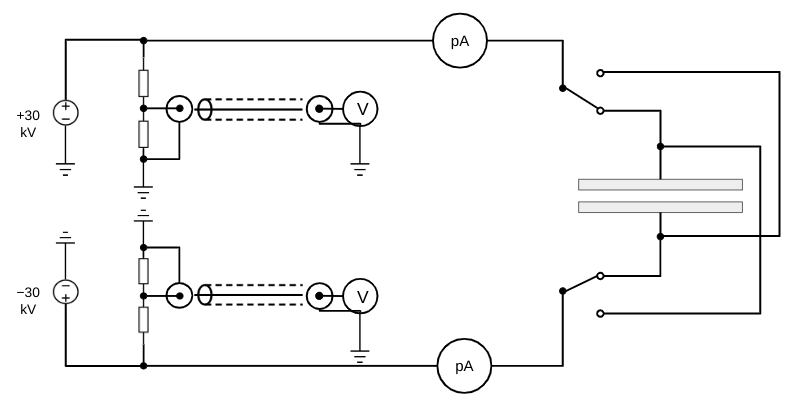
\includegraphics[width=\textwidth]{figs/todo/standard.png}
    \caption{The `standard' voltage measurement scheme.}
    \label{standard}
\end{figure}

Besides the voltage divider and voltmeter limitations discussed above, this
method is particularly sensitive to thermoelectric voltages that can develop at
all the low-voltage interfaces: between the resistor and the connector, between
the connector and the cable (on both sides of the cable), between the connector
and the voltmeter. As explained previously, these voltages (of order 5~$\mu$V/K)
are significant at the scale of the low voltages measured.

The problems associated with the thermocouple voltages can be avoided 

\begin{figure}
    \centering
    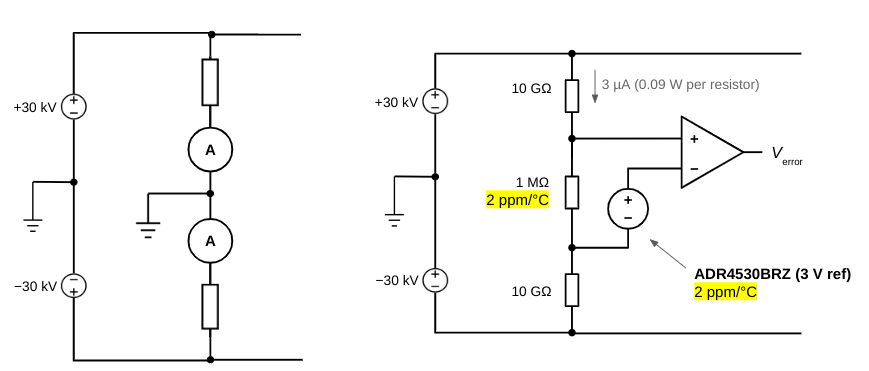
\includegraphics[width=\textwidth]{figs/todo/ammeter.png}
    \caption[The `ammeter' voltage measurement scheme.]{The `ammeter' voltage
    measurement scheme. \part{Left} Using two ammeters to monitor each polarity.
    \part{Right} Using a 1~M$\Omega$ single resistor to measure the entire
    voltage span.}
    \label{ammeter}
\end{figure}

\subsection{Voltage control}

\subsubsection{Lens HV control box}
